\documentclass{standalone}

\usepackage{circuitikz}

\begin{document}
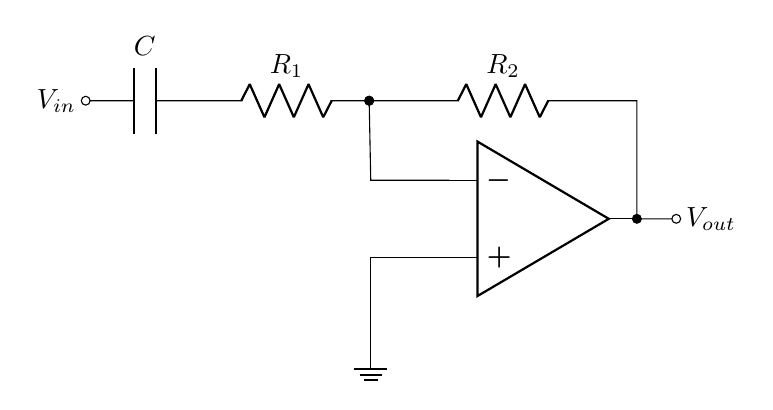
\begin{tikzpicture}
	\node[op amp, yscale=1] (opamp) at (-4,-0.5) {};
    \draw ($(opamp.out)+(-7,1.5)$) node[left] {$V_{in}$} 
    to[C, l=$C$, o-] ($(opamp.out)+(-5.5,1.5)$)
    to[R, l=$R_1$, -*] ($(opamp.out)+(-3.4,1.5)$) node (nodebetween1) {}
    to[R, l=$R_2$, *-]  ($(opamp.out)+(0,1.5)$) to[short] (opamp.out);
    \draw (nodebetween1.center) to[short] ($(opamp.-)+(-1,0)$)
    to[short] (opamp.-);
	%to[R, l=$R_2$, *-*] ($(opamp.out)+(0,+1.5)$) 
	%to[short] (opamp.out);
    \draw ($(opamp.+)$) to ($(opamp.+)+(-1,0)$) to ($(opamp.+)+(-1,-1)$) node [ground] {};
    \draw (opamp.out) to[short, *-o]  ($(opamp.out)+(0.5,0)$) node[right] {$V_{out}$};
\end{tikzpicture}
\end{document}